

\section{Comparison with other calibration methods {\color{blue} Laurence}}
\label{se:photometry_others}

The baseline results are compared to
results drawn using other calibration methods that either resort to different
opacity correction or include a photometric correction to correct for
the beam impact.

\begin{figure}[ht!]
  \begin{center}
    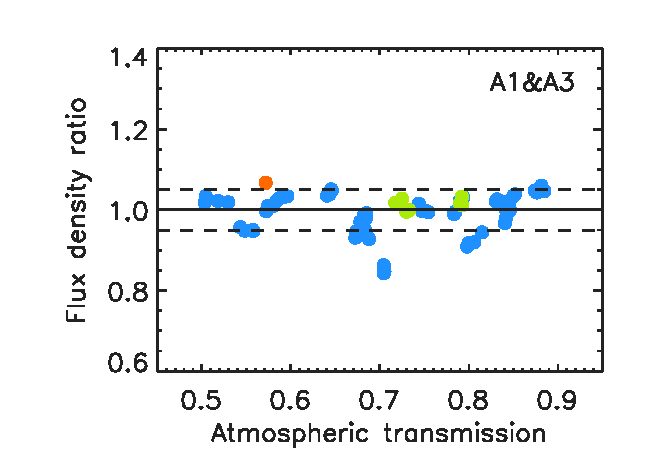
\includegraphics[clip=true, trim={0.9cm, 0.2cm, 0, 0.6cm},width=0.38\textwidth]{Figures/Calibration/plot_flux_density_ratio_MWC349_obstau_corrected_skydip_narrow_1mm.pdf}
    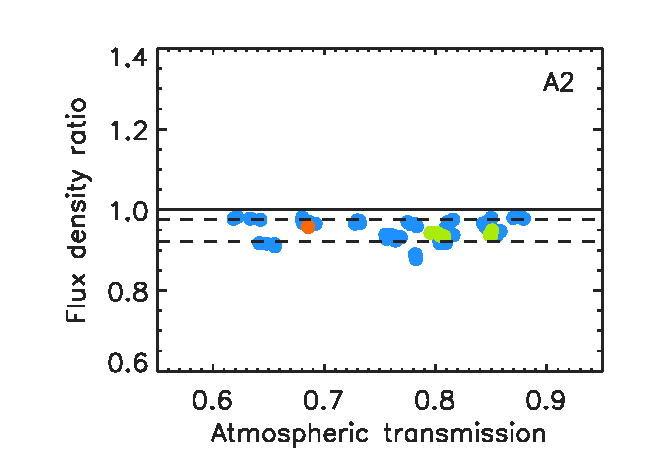
\includegraphics[clip=true, trim={0.9cm, 0.2cm, 0, 0.6cm},width=0.38\textwidth]{Figures/Calibration/plot_flux_density_ratio_MWC349_obstau_corrected_skydip_narrow_a2.pdf}
    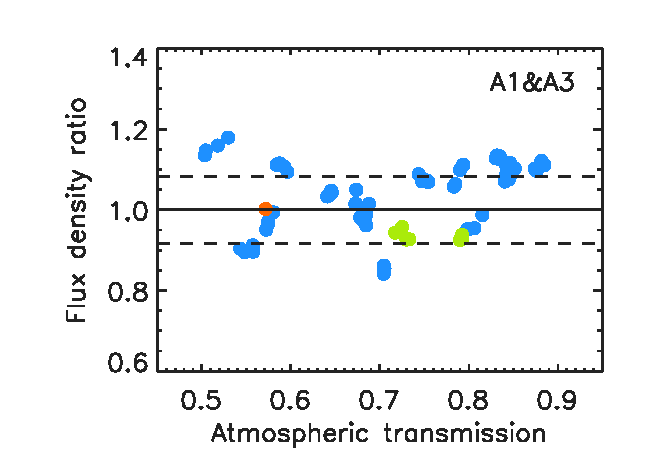
\includegraphics[clip=true, trim={0.9cm, 0.2cm, 0, 0.6cm},width=0.38\textwidth]{Figures/Calibration/plot_flux_density_ratio_MWC349_obstau_tau225_narrow_1mm.pdf}
    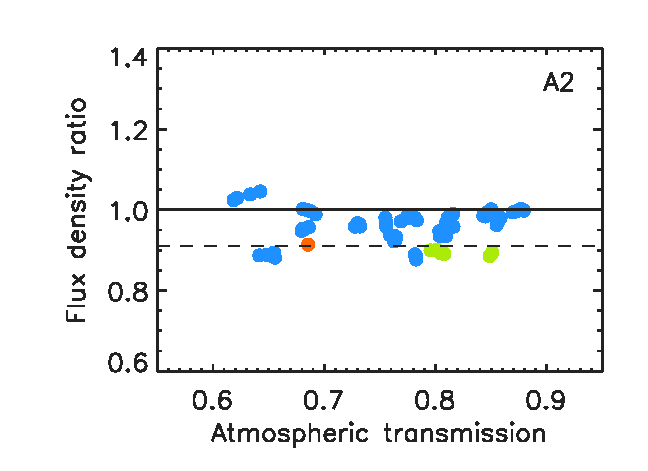
\includegraphics[clip=true, trim={0.9cm, 0.2cm, 0, 0.6cm},width=0.38\textwidth]{Figures/Calibration/plot_flux_density_ratio_MWC349_obstau_tau225_narrow_a2.pdf}
    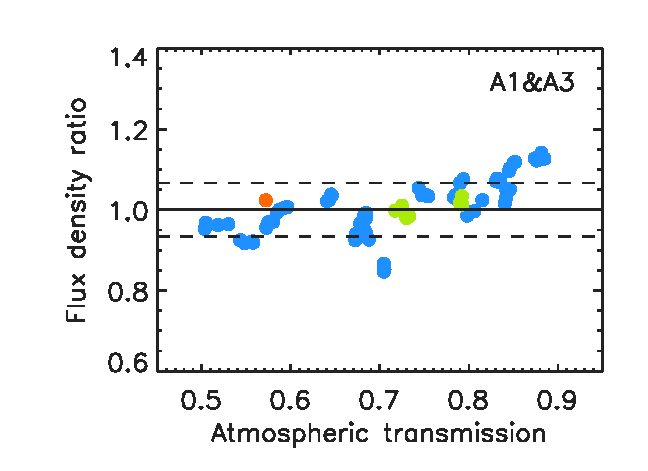
\includegraphics[clip=true, trim={0.9cm, 0.2cm, 0, 0.6cm},width=0.38\textwidth]{Figures/Calibration/plot_flux_density_ratio_MWC349_obstau_skydip_narrow_1mm.pdf}
    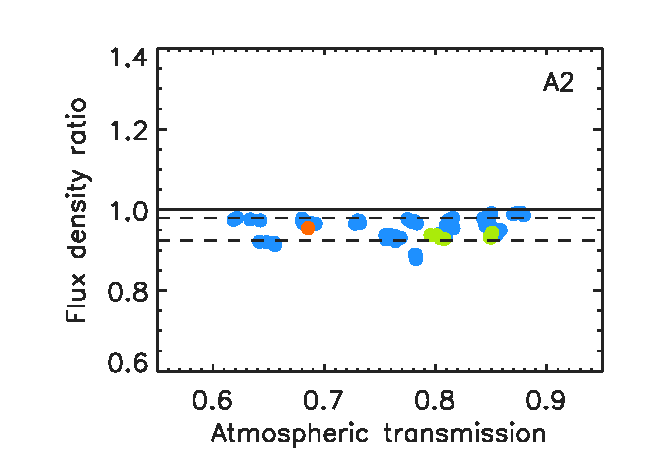
\includegraphics[clip=true, trim={0.9cm, 0.2cm, 0, 0.6cm},width=0.38\textwidth]{Figures/Calibration/plot_flux_density_ratio_MWC349_obstau_skydip_narrow_a2.pdf}
    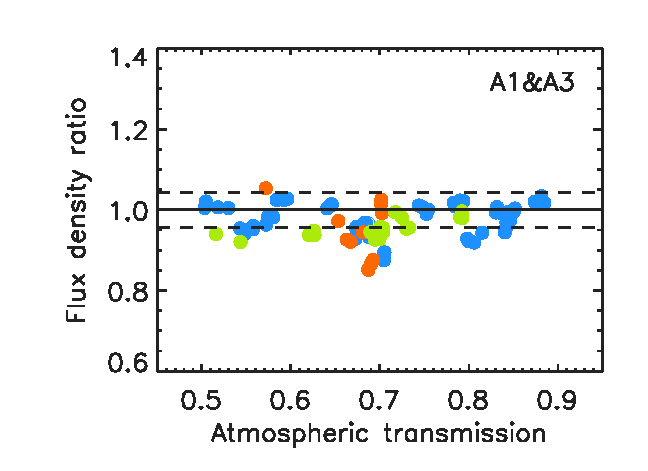
\includegraphics[clip=true, trim={0.9cm, 0.2cm, 0, 0.6cm},width=0.38\textwidth]{Figures/Calibration/plot_flux_density_ratio_MWC349_obstau_corrected_skydip_photocorr_demo_narrow_1mm.pdf}
    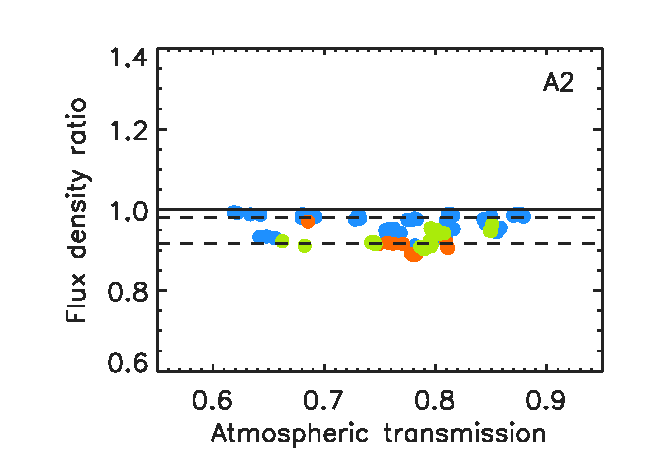
\includegraphics[clip=true, trim={0.9cm, 0.2cm, 0, 0.6cm},width=0.38\textwidth]{Figures/Calibration/plot_flux_density_ratio_MWC349_obstau_corrected_skydip_photocorr_demo_narrow_a2.pdf}
    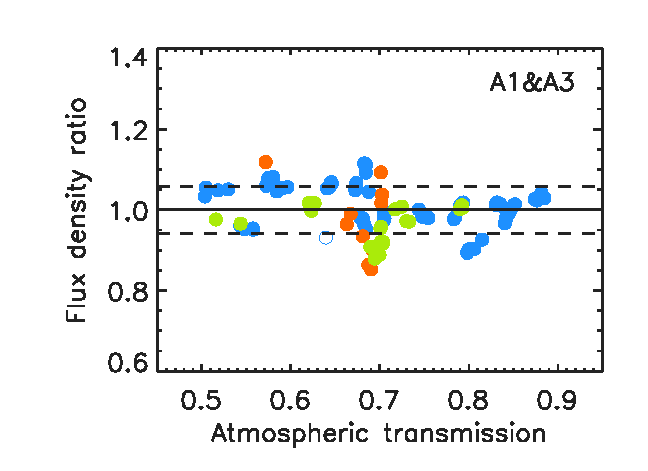
\includegraphics[clip=true, trim={0.9cm, 0.2cm, 0, 0.6cm},width=0.38\textwidth]{Figures/Calibration/plot_flux_density_ratio_MWC349_obstau_corrected_skydip_photocorr_pointing_narrow_1mm.pdf}
    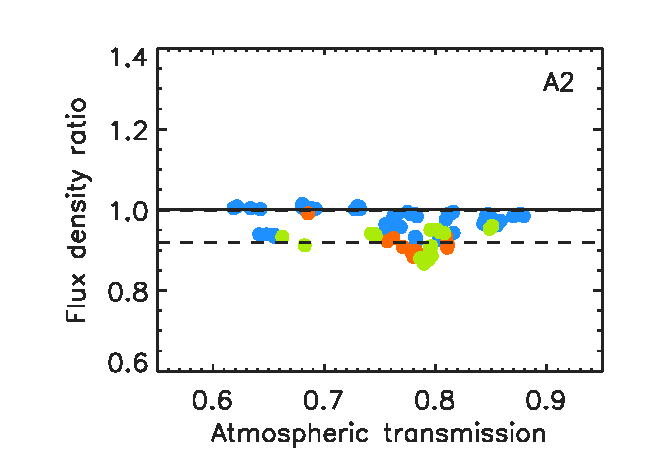
\includegraphics[clip=true, trim={0.9cm, 0.2cm, 0, 0.6cm},width=0.38\textwidth]{Figures/Calibration/plot_flux_density_ratio_MWC349_obstau_corrected_skydip_photocorr_pointing_narrow_a2.pdf}
    \caption[Calibration bias comparison]{Comparison of the
      calibration bias for five calibratio methods. The measured-to-expected flux density ratio is shown as a
      function of the atmospheric transmission for the baseline method
      (first row) as well as for methods using the 'taumeter' (second
      row) and 'skydip' (third) opacity correction, and for methods
      resorting to the 'demo' (fourth) and 'pointing' (fifth)
      photometric correction. Dashed lines
      show the flux density ratio $1 \sigma $ dispersion.}
    \label{fig:mwc349_obstau_others}
  \end{center}
\end{figure}


\begin{figure}[ht!]
  \begin{center}
    % baseline
    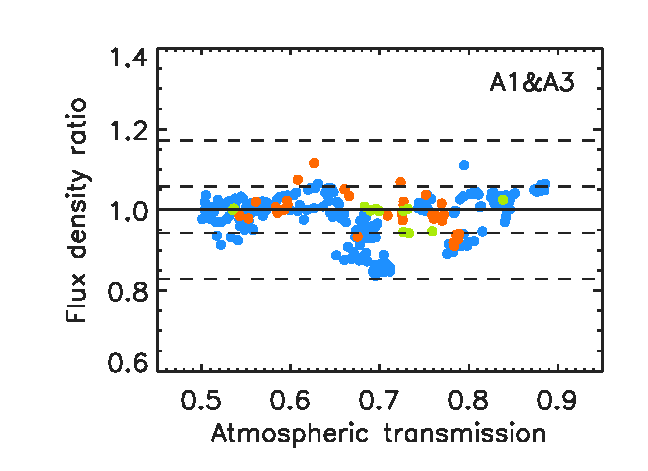
\includegraphics[clip=true, trim={0.9cm, 0.2cm, 0, 0.6cm}, width=0.32\textwidth]{Figures/Calibration/plot_flux_density_ratio_obstau_allbright_corrected_skydip_narrow_1mm.pdf}
    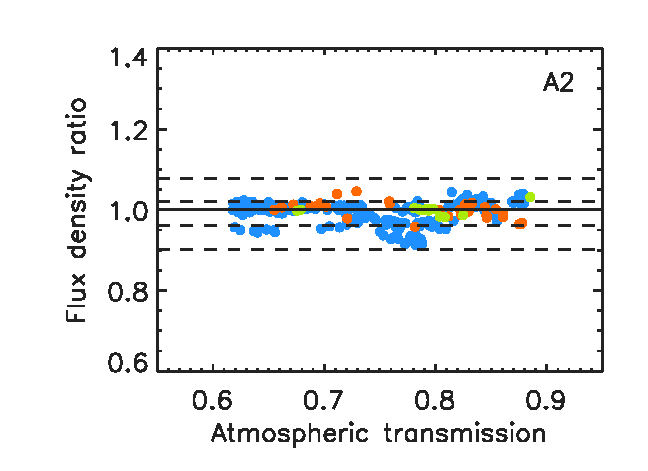
\includegraphics[clip=true, trim={0.9cm, 0.2cm, 0, 0.6cm}, width=0.32\textwidth]{Figures/Calibration/plot_flux_density_ratio_obstau_allbright_corrected_skydip_narrow_a2.pdf}
    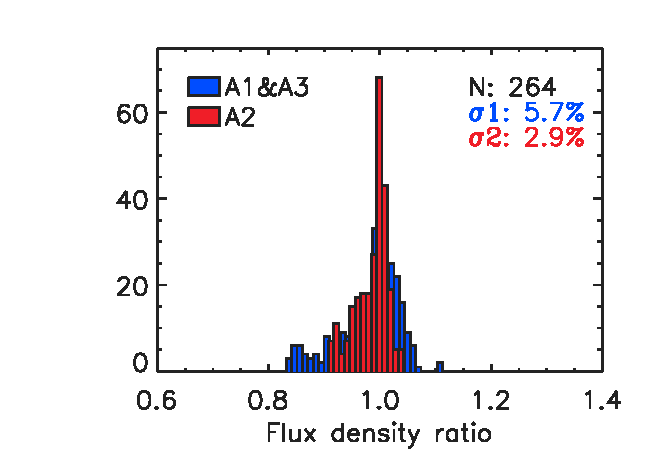
\includegraphics[clip=true, trim={0.9cm, 0.2cm, 0, 0.6cm}, width=0.32\textwidth]{Figures/Calibration/plot_histo_flux_density_ratio_obstau_allbright_corrected_skydip_narrow_1n2mm.pdf}
    % taumeter
    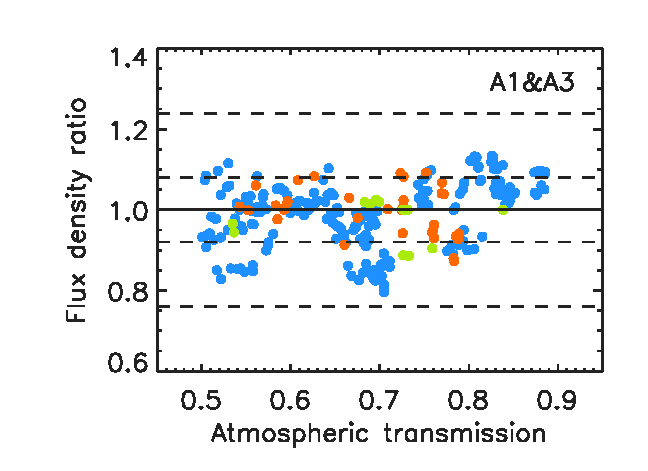
\includegraphics[clip=true, trim={0.9cm, 0.2cm, 0, 0.6cm}, width=0.32\textwidth]{Figures/Calibration/plot_flux_density_ratio_obstau_allbright_tau225_narrow_1mm.pdf}
    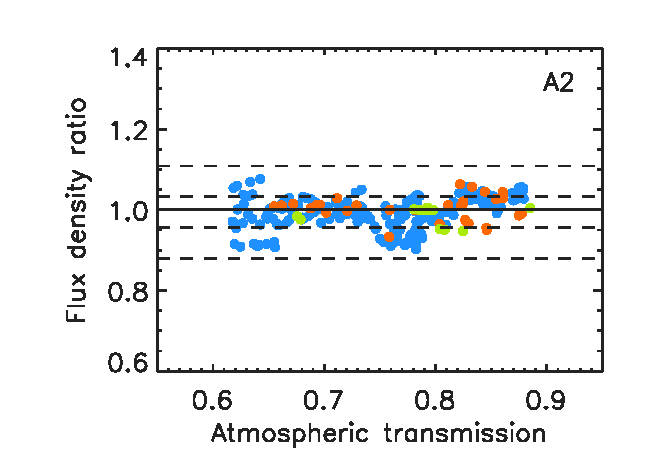
\includegraphics[clip=true, trim={0.9cm, 0.2cm, 0, 0.6cm}, width=0.32\textwidth]{Figures/Calibration/plot_flux_density_ratio_obstau_allbright_tau225_narrow_a2.pdf}
    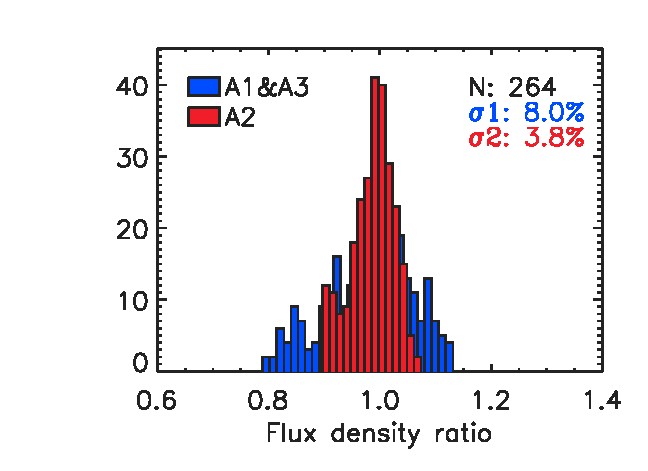
\includegraphics[clip=true, trim={0.9cm, 0.2cm, 0, 0.6cm}, width=0.32\textwidth]{Figures/Calibration/plot_histo_flux_density_ratio_obstau_allbright_tau225_narrow_1n2mm.pdf}
    % skydip
    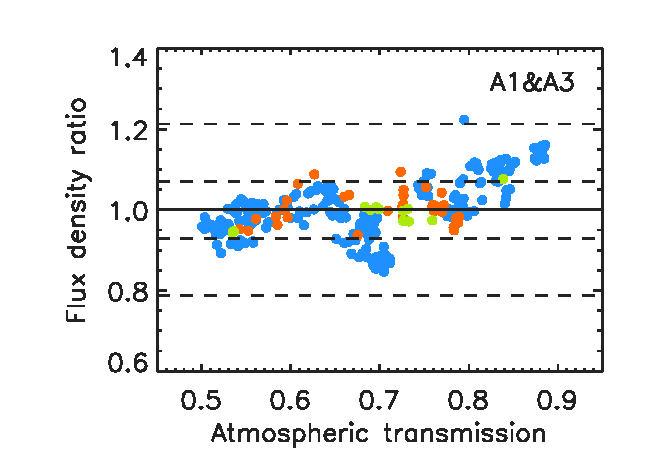
\includegraphics[clip=true, trim={0.9cm, 0.2cm, 0, 0.6cm}, width=0.32\textwidth]{Figures/Calibration/plot_flux_density_ratio_obstau_allbright_skydip_narrow_1mm.pdf}
    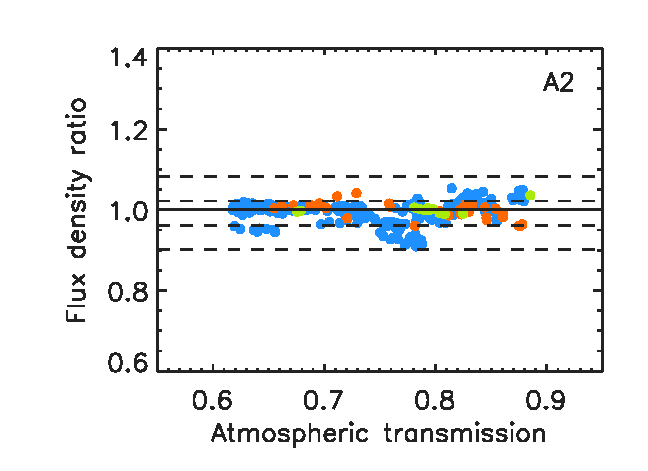
\includegraphics[clip=true, trim={0.9cm, 0.2cm, 0, 0.6cm}, width=0.32\textwidth]{Figures/Calibration/plot_flux_density_ratio_obstau_allbright_skydip_narrow_a2.pdf}
    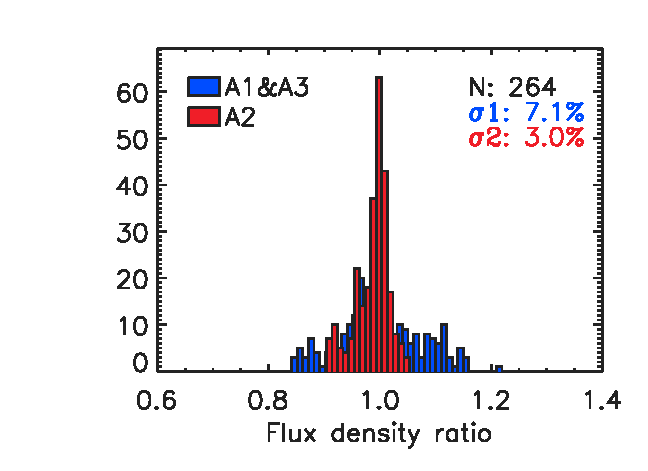
\includegraphics[clip=true, trim={0.9cm, 0.2cm, 0, 0.6cm}, width=0.32\textwidth]{Figures/Calibration/plot_histo_flux_density_ratio_obstau_allbright_skydip_narrow_1n2mm.pdf}
    % photocorr demo
    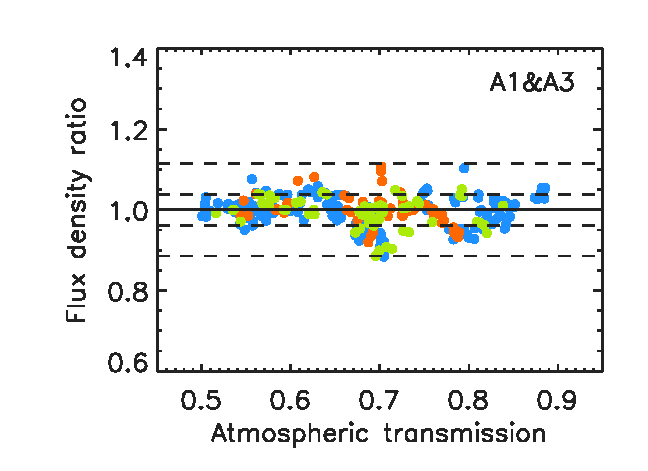
\includegraphics[clip=true, trim={0.9cm, 0.2cm, 0, 0.6cm}, width=0.32\textwidth]{Figures/Calibration/plot_flux_density_ratio_obstau_allbright_corrected_skydip_photocorr_demo_narrow_1mm.pdf}
    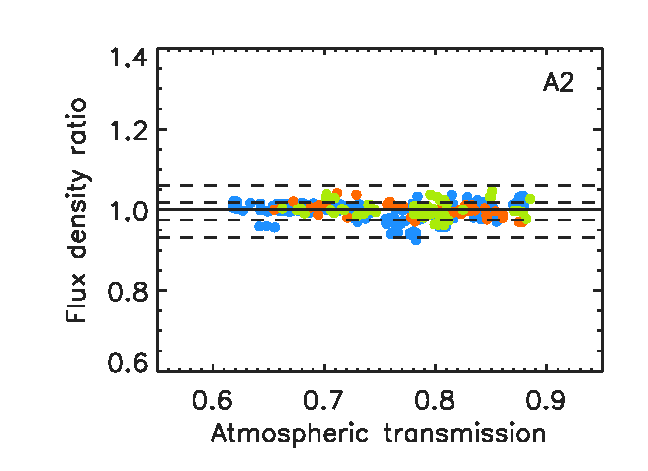
\includegraphics[clip=true, trim={0.9cm, 0.2cm, 0, 0.6cm}, width=0.32\textwidth]{Figures/Calibration/plot_flux_density_ratio_obstau_allbright_corrected_skydip_photocorr_demo_narrow_a2.pdf}
    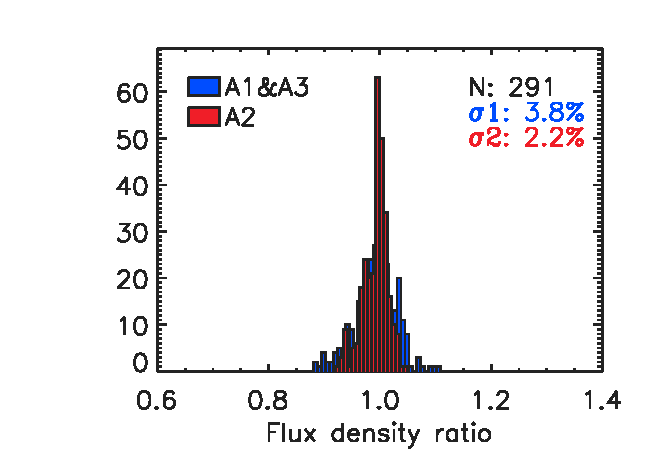
\includegraphics[clip=true, trim={0.9cm, 0.2cm, 0, 0.6cm}, width=0.32\textwidth]{Figures/Calibration/plot_histo_flux_density_ratio_obstau_allbright_corrected_skydip_photocorr_demo_narrow_1n2mm.pdf}
    % photocorr pointing
    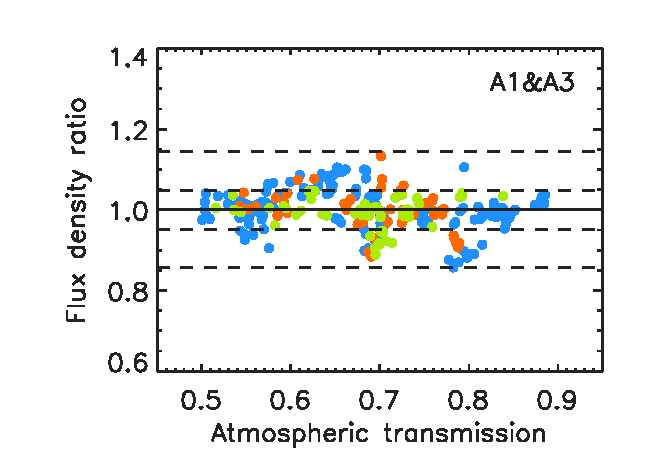
\includegraphics[clip=true, trim={0.9cm, 0.2cm, 0, 0.6cm}, width=0.32\textwidth]{Figures/Calibration/plot_flux_density_ratio_obstau_allbright_corrected_skydip_photocorr_pointing_narrow_1mm.pdf}
    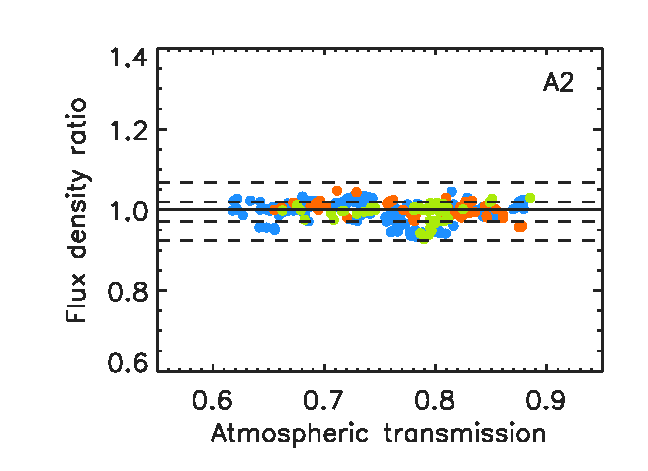
\includegraphics[clip=true, trim={0.9cm, 0.2cm, 0, 0.6cm}, width=0.32\textwidth]{Figures/Calibration/plot_flux_density_ratio_obstau_allbright_corrected_skydip_photocorr_pointing_narrow_a2.pdf}
    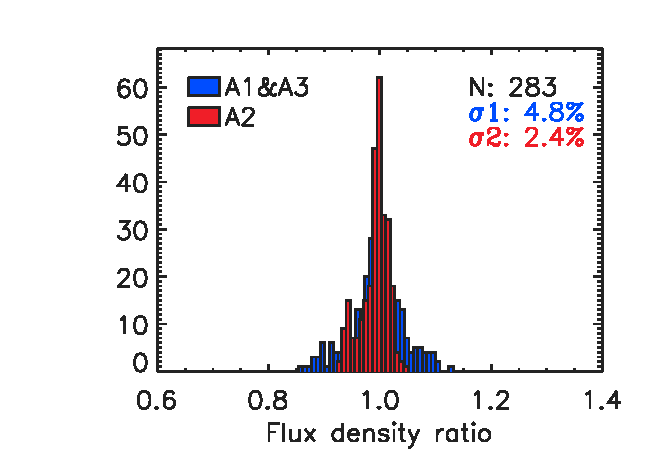
\includegraphics[clip=true, trim={0.9cm, 0.2cm, 0, 0.6cm}, width=0.32\textwidth]{Figures/Calibration/plot_histo_flux_density_ratio_obstau_allbright_corrected_skydip_photocorr_pointing_narrow_1n2mm.pdf}
    \caption[Comparison of calibration rms errors]{Comparison of the calibration uncertainties for five calibration methods. The
      measured-to-median flux density ratio at $1~\rm{mm}$ (first column) and $2~\rm{mm}$ (second column) of bright sources vs
      atmospheric transmission are shown as well as the flux density distibutions, using (first row) the baseline calibration, methods relying on (second row) the 'taumeter' and (third row) the 'skydip' opacity correction, and methods resorting to (fourth) row the 'demo' and (fifth row) the 'pointing' photometric correction.}
    \label{fig:allbright_rms_others}
  \end{center}
\end{figure}

    




%  COMBINED
%%%%%%%%%%%%%%%%%%%%%%%%%%%%%%%%%%%%%%%%%%%%%%%%%%%%%%%%%%%%%%%%%%
\begin{table}[th]
\begin{center}
\begin{tabular}{|c|l|c|c|c|c|c|}
  \hline
  \multicolumn{2}{|c|}{}  &  \multicolumn{5}{|c|}{Methods} \\\cline{3-7}
  \multicolumn{2}{|c|}{Characteristics} &  baseline  & taumeter  &  skydip  &  photocorr demo & photocorr pointing \\
  \hline\hline
  Bias &  $\#$ total    &   109   &   109    &   109    &    109    &  109   \\
       &  $\#$ selected &    72   &   72     &    72    &     96    &   95   \\
       &  A1            &   0.98  &  1.01    &  0.99    &   0.96    &  0.99  \\
       &  A3            &   1.00  &  1.03    &  1.01    &   0.98    &  1.01  \\
       &  1mm           &   0.99  &  1.02    &  1.00    &   0.97    &  1.00  \\
       &  2mm           &   0.95  &  0.96    &  0.95    &   0.95    &  0.96  \\
  \hline
  Rms  &  $\#$ total    &   487    &    487   &    487    &    396    &  396 \\
       &  $\#$ selected &   264    &    264   &    264    &    291    &  283 \\
       &  A1            &   5.5    &    7.5   &    7.3    &    3.9    &  4.8 \\
       &  A3            &   6.1    &    8.2   &    7.1    &    4.0    &  5.2 \\
       &  1mm           &   5.7    &    8.0   &    7.1    &    3.8    &  4.8 \\
       &  2mm           &   2.9    &    3.8   &    3.0    &    2.2    &  2.4 \\
\hline\hline
\end{tabular}
\caption[Summary table for a combination of all runs]{Combined}
\label{tab:Combined}
\end{center}
\end{table}

